\documentclass[final,5p]{elsarticle}

% \documentclass[preprint,12pt]{elsarticle}

%% Use the option review to obtain double line spacing
%% \documentclass[authoryear,preprint,review,12pt]{elsarticle}

%% Use the options 1p,twocolumn; 3p; 3p,twocolumn; 5p; or 5p,twocolumn
%% for a journal layout:
% \documentclass[final,1p,times]{elsarticle}
%% \documentclass[final,1p,times,twocolumn]{elsarticle}
% \documentclass[final,3p,times]{elsarticle}
%% \documentclass[final,3p,times,twocolumn]{elsarticle}
% \documentclass[final,5p,times]{elsarticle}
%% \documentclass[final,5p,times,twocolumn]{elsarticle}
\usepackage[portuguese]{babel}

%% For including figures, graphicx.sty has been loaded in
%% elsarticle.cls. If you prefer to use the old commands
%% please give \usepackage{epsfig}

%% The amssymb package provides various useful mathematical symbols
\usepackage{amssymb}
\usepackage{amsmath}
\usepackage{multirow}
\usepackage{tabularx}

\usepackage{pgfplots}
\pgfplotsset{compat=1.18}
\usepgfplotslibrary{statistics}
\usepackage{pgfplotstable}

\usepackage{placeins}
\usepackage{hyperref}
\numberwithin{equation}{section}

\usepackage{algorithm}
\usepackage[noEnd=true, indLines=true]{algpseudocodex}
\algrenewcommand\algorithmicrequire{\textbf{Entrada:}}
\algrenewcommand\algorithmicwhile{\textbf{Enquanto}}
\algrenewcommand\algorithmicrepeat{\textbf{Repete}}
\algrenewcommand\algorithmicuntil{\textbf{Até}}
\algrenewcommand\algorithmicif{\textbf{Se}}
\algrenewcommand\algorithmicthen{\textbf{então}}
\algrenewcommand\algorithmicelse{\textbf{Caso contrário}}
\algrenewcommand\algorithmicensure{\textbf{Objetivo:}}
\algrenewcommand\algorithmicreturn{\textbf{Retorna:}}
\algrenewcommand\algorithmicdo{\textbf{faça}}
\algrenewcommand\algorithmicforall{\textbf{Para todos}}
\algnewcommand{\LineComment}[1]{\State \(\triangleright\) \textcolor{black!50}{\emph{#1}}}

\newcommand*{\squareb}{\textcolor{black}{\rule{0.5em}{0.5em}}}
\newcommand*{\squareg}{\textcolor{gray}{\rule{0.5em}{0.5em}}}

\graphicspath{ {./png/} }

% \usepackage[fleqn]{nccmath}
% \usepackage{multicol}


%=========== Gloabal Tikz settings
% \pgfplotsset{compat=newest}
% \usetikzlibrary{math}
% \pgfplotsset{
%     height = 10cm,
%     width = 10cm,
%     tick pos = left,
%     legend style={at={(0.98,0.30)}, anchor=east},
%     legend cell align=left,
%     }
%  \pgfkeys{
%     /pgf/number format/.cd,
%     fixed,
%     precision = 1,
%     set thousands separator = {}
% }

%% The amsthm package provides extended theorem environments
%% \usepackage{amsthm}

%% The lineno packages adds line numbers. Start line numbering with
%% \begin{linenumbers}, end it with \end{linenumbers}. Or switch it on
%% for the whole article with \linenumbers.
%% \usepackage{lineno}

\usepackage{listings}
\usepackage{xcolor}

\definecolor{codegreen}{rgb}{0,0.6,0}
\definecolor{codegray}{rgb}{0.5,0.5,0.5}
\definecolor{codepurple}{rgb}{0.58,0,0.82}
\definecolor{backcolour}{rgb}{0.98,0.98,0.98}

\lstdefinestyle{mystyle}{
    backgroundcolor=\color{backcolour},
    commentstyle=\color{codegreen},
    keywordstyle=\color{magenta},
    numberstyle=\tiny\color{codegray},
    stringstyle=\color{codepurple},
    basicstyle=\ttfamily\footnotesize,
    breakatwhitespace=false,
    breaklines=true,
    captionpos=b,
    keepspaces=true,
    numbers=left,
    numbersep=5pt,
    showspaces=false,
    showstringspaces=false,
    showtabs=false,
    tabsize=2
}

\lstset{style=mystyle}

% \journal{Nuclear Physics B}

\begin{document}

\begin{frontmatter}

%% Title, authors and addresses

%% use the tnoteref command within \title for footnotes;
%% use the tnotetext command for theassociated footnote;
%% use the fnref command within \author or \address for footnotes;
%% use the fntext command for theassociated footnote;
%% use the corref command within \author for corresponding author footnotes;
%% use the cortext command for theassociated footnote;
%% use the ead command for the email address,
%% and the form \ead[url] for the home page:
%% \title{Title\tnoteref{label1}}
%% \tnotetext[label1]{}
%% \author{Name\corref{cor1}\fnref{label2}}
%% \ead{email address}
%% \ead[url]{home page}
%% \fntext[label2]{}
%% \cortext[cor1]{}
%% \affiliation{organization={},
%%             addressline={},
%%             city={},
%%             postcode={},
%%             state={},
%%             country={}}
%% \fntext[label3]{}

\title{Aplicação de Regressão Linear a Série Temporal\tnoteref{label_title}}
\tnotetext[label_title]{Relatório número 01 como parte dos requisitos da disciplina IA048: Aprendizado de Máquina.}

%% use optional labels to link authors explicitly to addresses:
%% \author[label1,label2]{}
%% \affiliation[label1]{organization={},
%%             addressline={},
%%             city={},
%%             postcode={},
%%             state={},
%%             country={}}
%%
%% \affiliation[label2]{organization={},
%%             addressline={},
%%             city={},
%%             postcode={},
%%             state={},
%%             country={}}

\author[label1]{Tiago C A Amorim (RA: 100675)}
\affiliation[label1]{organization={Doutorando no Departamento de Engenharia de Petróleo da Faculdade de Engenharia Mecânica, UNICAMP},
            city={Campinas},
            state={SP},
            country={Brasil}}

\author[label2]{Taylon L C Martins (RA: 177379)}
\affiliation[label2]{organization={Aluno especial, UNICAMP},
            city={Campinas},
            state={SP},
            country={Brasil}}


% \begin{abstract}

%     xxxxxxx

% \end{abstract}


%%Graphical abstract
% \begin{graphicalabstract}
%\includegraphics{grabs}
% \end{graphicalabstract}

%%Research highlights
% \begin{highlights}
% \item Research highlight 1
% \item Research highlight 2
% \end{highlights}

\begin{keyword}
    Regressão Linear \sep Séries Temporais \sep Validação Cruzada
%% keywords here, in the form: keyword \sep keyword

%% PACS codes here, in the form: \PACS code \sep code

%% MSC codes here, in the form: \MSC code \sep code
%% or \MSC[2008] code \sep code (2000 is the default)

\end{keyword}

\end{frontmatter}

%% main text
\section{Introdução}

    Este relatório apresenta as principais atividades realizadas no desenvolvimento das atividades propostas na Lista 01 da disciplina IA048: Aprendizado de Máquina, primeiro semestre de 2024. O foco deste exercício é de construir modelos lineares para realizar a previsão de uma série temporal.

\section{Tarefa Proposta}

    Trabalhar com a base de dados U.S. Airline Traffic Data, a qual contém informações referentes ao tráfego aéreo mensal norte-americano no período de 2003 a 2023, disponibilizadas pelo \emph{U.S. Department of Transportation’s (DOT) Bureau of Transportation Statistics}. Em particular, vamos explorar a série temporal do número total de voos (domésticos e internacionais).

    Explorar um modelo linear para a previsão considerando que o horizonte de predição é L = 1 (passos à frente da série temporal).

    \begin{enumerate}[(a)]
        \item Exiba o gráfico da série temporal completa. Numa inspeção visual simples, é possível reconhecer ao menos três faixas distintas de comportamento aproximadamente “regular” na série:

        \begin{enumerate}[(i)]
            \item Jan/2003 a Ago/2008.
            \item Set/2008 a Dez/2019.
            \item Jan/2020 a Set/2023.
        \end{enumerate}

        Discuta possíveis razões históricas/econômicas para as transições de comportamento.

        \item Divida a série em dois conjuntos:

        \begin{enumerate}[(i)]
            \item \textbf{Treinamento} e \textbf{validação}: com amostras de 2003 a 2019.
            \item \textbf{Teste}: com amostras de 2020 a 2023.
        \end{enumerate}

        Faça a análise de desempenho do preditor linear ótimo, no sentido de quadrados mínimos irrestrito considerando:

        \begin{enumerate}[(1)]
            \item A progressão do valor da raiz quadrada do erro quadrático médio (RMSE, do inglês \emph{root mean squared error}), junto aos dados de validação, em função do número de entradas (\textbf{K}) do preditor (desde K = 1 a K = 24). Apresente o gráfico obtido e busque tecer conjecturas sobre os motivos subjacentes a seu comportamento. \label{item:b1}
            \item O gráfico com as amostras de teste da série temporal e as respetivas estimativas geradas pela melhor versão do preditor (i.e., usando o valor de \textbf{K} que levou ao mínimo erro de validação). Obtenha, também, o RMSE e o erro percentual absoluto médio (MAPE, do inglês \emph{mean absolute percentage error}) para o conjunto de teste.  \label{item:b2}
            \item O gráfico com as amostras apenas dos dois últimos anos (2022 e 2023) e as estimativas geradas pelo melhor preditor, além dos respetivos valores de RMSE e MAPE.  \label{item:b3}
        \end{enumerate}

        \item Repita o procedimento detalhado nos itens \ref{item:b1} e \ref{item:b2}, mas adotando a seguinte divisão dos dados:

        \begin{enumerate}[(i)]
            \item \textbf{Treinamento}: amostras de 2003 a 2019.
            \item \textbf{Validação}: amostras de 2020 e 2021.
            \item \textbf{Teste}: amostras de 2022 e 2023.
        \end{enumerate}

        Discuta os resultados obtidos e faça uma comparação com o cenário anterior (especialmente
        com o que foi obtido no item \ref{item:b3}).
    \end{enumerate}

\section{Aplicação}

    Toda a avaliação foi feita em um único \emph{notebook} Jupyter, em Python. Foi feito o uso da biblioteca \emph{Scikit-learn} \cite{scikit-learn} para fazer as diferentes manipulações nos dados. O código pode ser encontrado em \href{https://github.com/TiagoCAAmorim/machine_learning/blob/main/Lista01/Lista01.ipynb}{https://github.com/Tiago CAAmorim/machine\_learning}.

    \subsection{Avaliação do Conjunto de Dados}

    O conjunto de dados utilizado nesta avaliação é o de tráfego aéreo dos EUA disponibilizado no Kaggle \cite{YYXian_2024}. Segundo o autor este conjunto de dados fornece o tráfego aéreo mensal dos EUA de 2003 a 2023, incluindo o número de passageiros, o número de voos, as milhas de passageiros pagantes, as milhas de assentos disponíveis e o fator de ocupação.

    Nesta avaliação o foco é no número total de voos. A figura \ref{fig:principal} mostra que o período de janeiro/2003 a agosto/2008 (azul) é de certa normalidade na economia americana. O início do período em verde (setembro/2008) é marcado pelo início da crise financeira do \emph{subprime}. Esta crise foi consequência do estouro da bolha imobiliária nos EUA devido a empréstimos sem lastro e preços de imóveis inflacionados. O período em vermelho corresponde à crise sanitária causada pela pandemia de Covid-19 e os anos que se seguiram. A queda mais significativa, que inicia em janeiro/2020, corresponde ao período de maior restrição de voos imposta durante a crise sanitária.

    \begin{figure}[hbt!]
        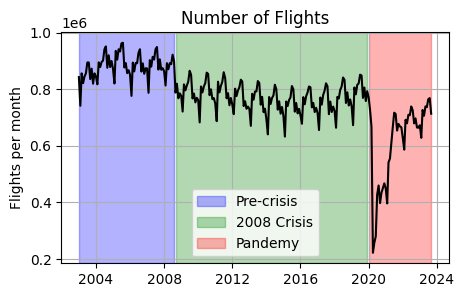
\includegraphics[width=0.95\columnwidth]{A_MainSeries.png}
        \caption{Série com total de voos nos EUA.}
        \label{fig:principal}
    \end{figure}

    \subsubsection{Pré-processamento}
    Alguns exemplos na figura \ref{fig:exemplo_original} mostram que a série original apresenta um caráter cíclico (com frequência anual) e \emph{serrilhado} (não-suave). Foram avaliadas duas alternativas para deixar a série temporal mais suave e facilitar o processo de regressão. Como os meses do ano não tem o mesmo número de dias, uma primeira tentativa foi de calcular o número médio de voos por dia para cada mês da série. A segunda tentativa foi de calcular o número de voos diários considerando apenas os dias úteis de cada mês.

    \begin{figure}[hbt!]
        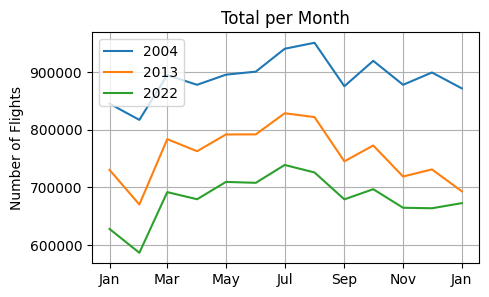
\includegraphics[width=0.95\columnwidth]{A_Total_per_Month.png}
        \caption{Exemplos de total de voos nos EUA ao longo do ano.}
        \label{fig:exemplo_original}
    \end{figure}

    A figura \ref{fig:exemplo_media} mostra que a série temporal de média diária de voos por mês se mostra mais suave que a série original. O efeito é mais pronunciado no mês de fevereiro. A série temporal de total mensal de voos dividido pelo número de dias úteis, na figura \ref{fig:exemplo_dais_uteis}, não teve uma reposta adequada.

    \begin{figure}[hbt!]
        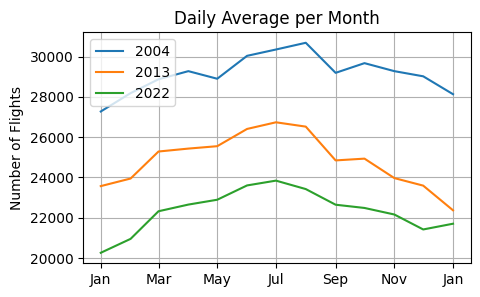
\includegraphics[width=0.95\columnwidth]{A_Daily_Average_per_Month.png}
        \caption{Exemplos de média diária do total de voos nos EUA.}
        \label{fig:exemplo_media}
    \end{figure}

    \begin{figure}[hbt!]
        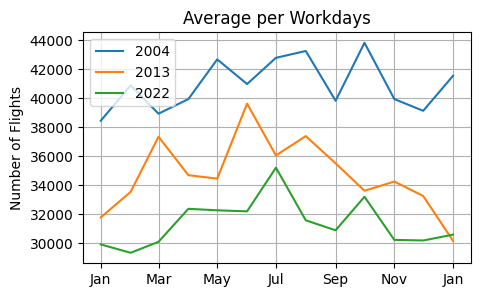
\includegraphics[width=0.95\columnwidth]{A_Average_per_Workdays.png}
        \caption{Exemplos do total de voos nos EUA pelo número de dias úteis no mês.}
        \label{fig:exemplo_dais_uteis}
    \end{figure}

    Optou-se por utilizar a média mensal de voos por dia nas análises posteriores (figura \ref{fig:serie_alternativa}). Todos os valores de RMSE e MAPE foram calculados em função desta nova série.

    \begin{figure}[hbt!]
        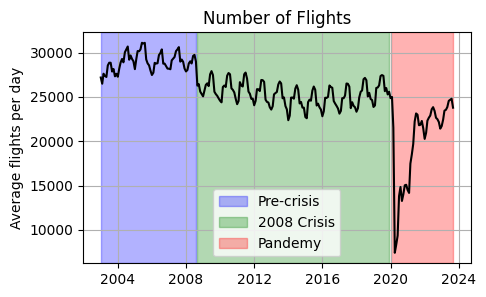
\includegraphics[width=0.95\columnwidth]{A_NewSeries.png}
        \caption{Média diária do total de voos nos EUA.}
        \label{fig:serie_alternativa}
    \end{figure}

    \subsection{Primeiro Modelo de Regressão}

    Antes de separar os dados em treino+validação e teste, foram construídas séries temporais com os valores passados associado a cada entrada na série de voos\footnote{Ao longo destes tópicos a série que se busca ajustar é a da média diária de voos.}. Definindo a série de média diária de voos como $\textbf{y}$, as séries dos valores passados foram definidas como:

    \begin{equation}
        \textbf{x}_{\textbf{k}}(t_i) = \textbf{y}(t_{i-k}) \quad \text{com} \; k=1,\ldots,24 \label{eq:definicao_xs}
    \end{equation}

    \noindent Onde $t_i$ são os índices dos dados da série temporal.

    De modo a ter uma melhor comparação entre os diferentes modelos que serão construídos, foram retiradas todas as linhas com valores não definidos (as 24 primeiras entradas da tabela de dados). Desta forma todos os processos de treino e validação são feitos com os mesmos conjuntos de dados. Com este filtro o total de dados passa de 249 para 225.

    Aplicando os limites propostos no item \ref{item:b1}, o conjunto de dados de treino+validação fica com 180 elementos e o de teste com 45. Os intervalos de dados de treino+validação e teste apresentam um comportamento cíclico, com suaves variações ao longo dos anos (figura \ref{fig:treino_teste}). A exceção no conjunto de treino+validação é no início de 2008, quando eclodiu a crise financeira nos EUA. O início do intervalo de teste corresponde ao período crítido de restrição de vôos da pandemia de Covid-19. É esperado que o modelo apresente dificuldades em prever a série temporal no período mais crítico da pandemia.

    \begin{figure}[hbt!]
        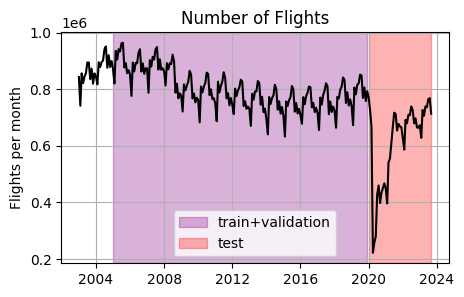
\includegraphics[width=0.95\columnwidth]{B1_TrainTest.png}
        \caption{Períodos de treino+validação e teste.}
        \label{fig:treino_teste}
    \end{figure}

    \subsubsection{Normalização dos Dados}

    Como todas as variáveis de entrada dos modelos lineares são de mesma natureza, uma modificação na escala dos dados não tem qualquer impacto nos resultados dos ajustes dos modelos lineares. Foi realizado um rápido teste assumindo um modelo linear sem regularização. Como conjunto de teste foram utilizados os primeiros 140 dados do conjunto de treino+validação, e os demais como conjunto de validação. Foram utilizados $\textbf{x}_{\textbf{1}}$ e $\textbf{x}_{\textbf{2}}$ como variáveis do problema.

    A tabela \ref{tab:efeito_mimmaxscaler} mostra que, mesmo gerando modelos distintos, os resultados de RMSE são os mesmos quando as variáveis de entrada estão no intervalo $[0;1]$\footnote{Foi utilizada a classe \textbf{MinMaxScaler} do \emph{Scikit-learn}} e quando estão com os valores originais.

    \begin{table}[h]
        \centering
        \begin{tabular}{l c c}
        \hline
        RMSE & Valores & Com Mudança \\
         & Originais & de Escala \\
        \hline
        Treino & 788.91 & 788.91 \\
        Validação & 854.33 & 854.33 \\
        \hline
        \end{tabular}
        \caption{Efeito da normalização dos dados de entrada.}
        \label{tab:efeito_mimmaxscaler}
    \end{table}

    Durante as iterações da rotina de busca do melhor modelo linear o algoritmo teve dificuldades de convergência com valores altos de \textbf{K} (>15). Ao modificar a escala dos dados de entrada o algoritmo não apresentou problemas. Deste modo, as análises seguintes foram feitas com os dados de entrada escalados para o intervalo $[0;1]$.

    \subsubsection{Validação Cruzada}

    Como existe dependência entre os dados observados, o processo de validação cruzada \emph{clássico}, que define os conjuntos de treino e validação sem levar em conta a sua ordem, não pode ser utilizado. Os dados de validação ($I(v)$) são definidos em índices posteriores aos dos dados de treinamento ($I(t)$) \cite{10.1214/09-SS054}:

    \begin{equation}
        \min{}_{i \epsilon I(t), j \epsilon I(v)} |i - j| > h > 0
    \end{equation}

    Foi utilizada a rotina \textbf{TimeSeriesSplit}, implementada no pacote \emph{Scikit-learn}, e um total de 4 pastas (\emph{folds}). A rotina do \emph{Scikit-learn} equivale a utilizar $h=1$. A figura \ref{fig:folds} mostra a divisão dos dados entre treino e validação para cada pasta.

    \begin{figure}[hbt!]
        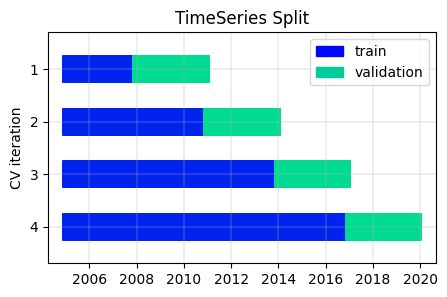
\includegraphics[width=0.95\columnwidth]{B1_Folds.png}
        \caption{Divisão entre treino e validação para cada pasta.}
        \label{fig:folds}
    \end{figure}

    \subsubsection{Modelos Simples} \label{sec:modelos_naive}

    Antes de seguir com o teste de diversos modelos lineares, foram propostos três modelos simples (\emph{naïve}):
    \begin{enumerate}
        \item Igual ao passo de tempo anterior:

        $\quad \hat{\textbf{y}}(t) = \textbf{y}(t-1)$

        \item Igual ao passo de tempo 12 meses atrás:

        $\quad \hat{\textbf{y}}(t) = \textbf{y}(t-12)$

        \item Igual ao passo de tempo 12 meses atrás mais variação entre 24 e 12 meses atrás:

        $\quad \hat{\textbf{y}}(t) = \textbf{y}(t-12) + [\textbf{y}(t-12) - \textbf{y}(t-24)]$
    \end{enumerate}

    Os modelos \emph{naïve} foram propostos com base na natureza cíclica da série temporal em estudo. Os valores de RMSE e MAPE destes modelos servirão como referência para os demais modelos a serem construídos.

    Foi aplicada validação cruzada a cada um dos modelos e computada a média dos RMSE. Os resultados de RMSE são relativamente próximos: $861.25$, $765.83$ e $950.38$, para o primeiro, segundo e terceiro modelos \emph{naïve} propostos, respectivamente. Em uma inspeção gráfica (figura \ref{fig:naive}) a primeira proposta de modelo parece ser melhor que as outras duas. Uma avaliação do gráfico do erro cometido por estes modelos (figura \ref{fig:naive_erros}) demonstra que na verdade os modelos tem níveis de erro parecidos, mas com diferentes frequências.

        \begin{figure}[hbt!]
            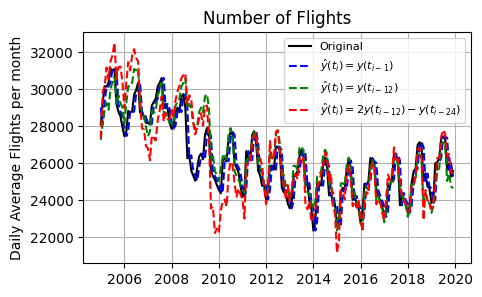
\includegraphics[width=0.95\columnwidth]{B1_Naive.png}
            \caption{Modelos simples (\emph{naïve}).}
            \label{fig:naive}
        \end{figure}

        \begin{figure}[hbt!]
            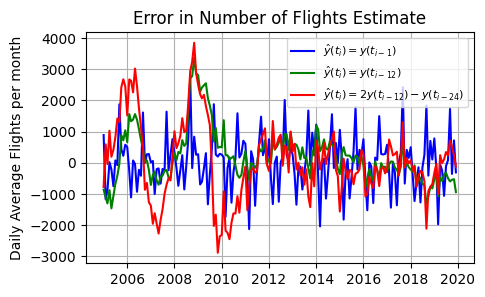
\includegraphics[width=0.95\columnwidth]{B1_NaiveErrors.png}
            \caption{Erros dos modelos simples.}
            \label{fig:naive_erros}
        \end{figure}

    O segundo modelo \emph{naïve} tem o menor valor de RMSE médio, e apresenta um gráfico de erro melhor \emph{comportado} que os demais. Este segundo modelo foi o escolhido para ser utilizado como referência na busca pelo modelo \emph{ótimo}.

    \subsubsection{Busca pelo Melhor Modelo}

    Em um primeiro momento foi definido utilizar um modelo linear regularizado do tipo \emph{Elastic-Net}:

    \begin{equation}
        \frac{1}{2 n} ||y - Xw||^2_2 + \alpha{} \, l1_{ratio} ||w||_1 + \frac{\alpha{}}{2} (1 - l1_{ratio}) ||w||^2_2
    \end{equation}

    \noindent Onde $n$ é o número de amostras e $w$ são os pesos do modelo linear.

    A busca pelo melhor modelo para cada valor de \textbf{K} foi feita com uma busca em grade (\emph{grid search}) por parâmetros ótimos de $\alpha{}$ (entre $0.01$ e $1.0$) e $l1_{ratio}$ (entre $0.1$ e $0.9$). O parâmetro de busca do melhor modelo foi a média do RMSE.

    Todos os 24 modelos encontrados utilizaram o menor valor de $\alpha{}$ que fez parte da busca em grade ($0.01$). Em face destes resultados a avaliação foi refeita utilizando um modelo linear simples (sem regularização). Como o novo modelo não tem parâmetros, não foi preciso realizar uma busca em grade, e foi testado apenas o valor de \textbf{K} (figura \ref{fig:modelos_lineares}).

    \begin{figure}[hbt!]
        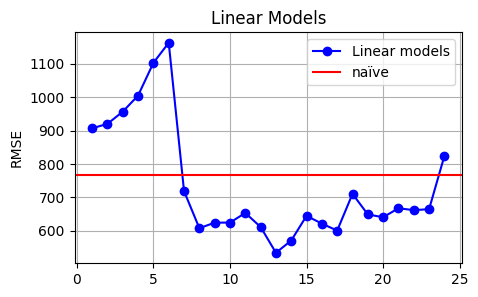
\includegraphics[width=0.95\columnwidth]{B1_LinearModels.png}
        \caption{RMSE de validação médio dos modelos lineares em função de \textbf{K}.}
        \label{fig:modelos_lineares}
    \end{figure}

    O melhor resultado foi com \textbf{K} igual a 13 (validação cruzada com $\text{RMSE} = 534.25$ e $\text{MAPE} = 0.02$). Com o melhor valor de \textbf{K} definido, foi utilizado todo o conjunto de dados de treino+validação para ajustar os parâmetros do modelo escolhido.

    Foi ajustado um segundo modelo com \textbf{K} igual a 13, mas sem normalizar as variáveis. Com este modelo fica mais fácil analisar os valores dos coeficientes do modelo. O modelo linear pode ser interpretado como uma média ponderada dos valores nos meses anteriores, já que as variáveis e o valor de saída tem todos a mesma natureza. A soma dos coeficientes com o valor relativo da constante\footnote{Foi definido valor relativo da constante como a divisão do termo constante do modelo linear pela média dos valores de saída.} é próxima da unidade: $0.9687 + 0.0305 = 0.9992$.

    A figura \ref{fig:coef_modelo_linear} mostra os valores dos coeficientes utilizados. As variáveis de maior peso foram o passo de tempo anterior ($\textbf{x}_{\textbf{1}}$), um ano antes ($\textbf{x}_{\textbf{12}}$) e o anterior ($\textbf{x}_{\textbf{13}}$). Este resultado guarda certa correspondência com dois dos modelos \emph{naïve} propostos, dando maior peso ao valor anterior (tendência de curto prazo) e ao valor um ano atrás (efeito da sazonalidade).

    \begin{figure}[hbt!]
        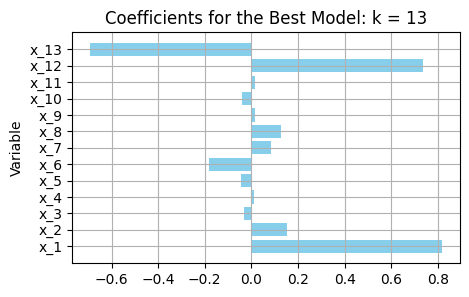
\includegraphics[width=0.95\columnwidth]{B1_CoefficientsNoScaling.png}
        \caption{Coeficientes do melhor modelo linear ($\textbf{K} = 13$).}
        \label{fig:coef_modelo_linear}
    \end{figure}


    \subsubsection{Erros com os Dados de Teste} \label{sec:testes_modelo}

    O modelo construído teve um resultado ruim nos dados de teste, com $\text{RMSE} = 3\,187.$ e $\text{MAPE} = 0.1126$. Na figura \ref{fig:melhor_modelo_teste} observa-se que o conjunto de teste (área em vermelho na figura) coincide com o período da pandemia e os meses posteriores. Por se tratar de um evento singular e que não apareceu nos dados de treino e validação, já era esperado que o modelo tivesse dificuldade em prever o comportamento da série temporal. O alto valor de RMSE associado ao conjunto de teste demonstra a dificuldade do modelo.

    \begin{figure}[hbt!]
        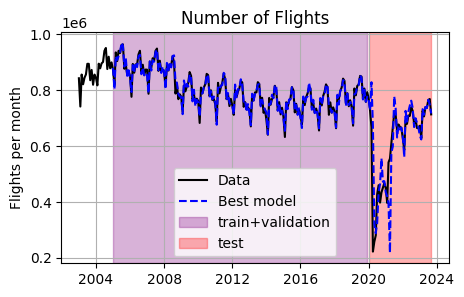
\includegraphics[width=0.95\columnwidth]{B2_BestModelFit.png}
        \caption{Ajuste do melhor modelo linear ($\textbf{K} = 13$).}
        \label{fig:melhor_modelo_teste}
    \end{figure}

    Quando o período de teste é limitado aos anos de 2022 e 2023 os resultados são bem melhores ($\text{RMSE} = 575.85$ e $\text{MAPE} = 0.0190$). O período de 2022 a 2023 corresponde ao final da pandemia de Covid-19, quando muitas das barreiras sanitárias já estavam sendo levantadas. O comportamento da série temporal neste intervalo já se assemelha mais ao comportamento observado nos dados de treino e validação (figura \ref{fig:melhor_modelo_2223}). Um valor de RMSE mais próximo do observado no processo de validação cruzada mostra que o modelo teve um resultado aceitável para este período (figura \ref{fig:erros_melhor_modelo}).

        \begin{figure}[hbt!]
            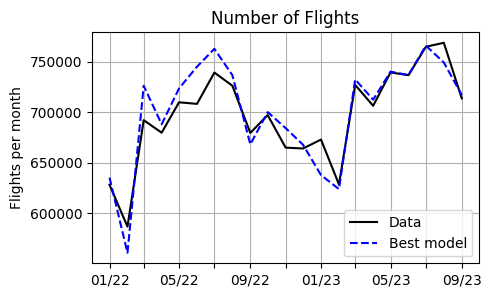
\includegraphics[width=0.95\columnwidth]{B3_BestModel22_23.png}
            \caption{Ajuste do melhor modelo linear ($\textbf{K} = 13$) ao anos de 2022 e 2023.}
            \label{fig:melhor_modelo_2223}
        \end{figure}

        \begin{figure}[hbt!]
            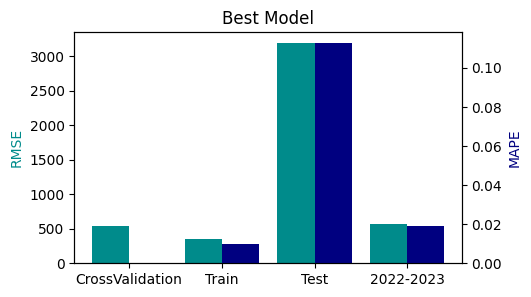
\includegraphics[width=0.95\columnwidth]{B3_RMSE.png}
            \caption{Resumo dos erros do melhor modelo linear ($\textbf{K} = 13$).}
            \label{fig:erros_melhor_modelo}
        \end{figure}

        \subsection{Segundo Modelo de Regressão}

        Para o segundo modelo de regressão a proposta é utilizar outros intervalos para treino, validação e teste (figura \ref{fig:treino_teste_modelo_dois}). O intervalo de validação coincide com o período de maior restrição de deslocamento da pandemia de Covid-19. Dada a discrepância entre o comportamento da série temporal no período de treino e no de validação, é esperado que as variáveis que correspondem a dados mais recentes tenham maior peso. Adicionalmente, como o intervalo de validação está fixo, não será possível fazer validação cruzada.

        \begin{figure}[hbt!]
            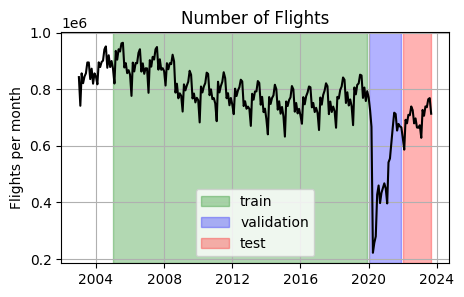
\includegraphics[width=0.95\columnwidth]{C1_TrainTest.png}
            \caption{Série temporal com novos limites dos dados de treino, validação e teste.}
            \label{fig:treino_teste_modelo_dois}
        \end{figure}

        Foram testados os mesmos modelos simples (\emph{naïve}) propostos anteriormente (em \ref{sec:modelos_naive}). O modelo de melhor resultado foi o que utiliza o valor do mês anterior para prever o próximo intervalo de tempo. Os resultados de RMSE foram $3\,304.$, $11\,023.$ e $17\,523.$, para o primeiro, segundo e terceiro modelos \emph{naïve} propostos, respectivamente. Como o intervalo de validação corresponde a um perído de significativas variações na série temporal, os modelos que se baseiam em horizontes de tempo mais longo tem mais dificuldade de prever este comportamento.

        O mesmo comportamento observado entre os modelos \emph{naïve} apareceu na seleção de modelos em função da quantidade de passos de tempo passados (figura \ref{fig:modelos_lineares_novo}). Os modelos que se restringem a dados de passos de tempo mais recentes apresentaram melhores resultados. Este resultado é devido ao conjunto de dados de validação utilizado. O melhor modelo é o que se baseia apenas nos dois passos de tempo anteriores, e com maior impacto do passo de tempo imediatamente anterior.

        \begin{figure}[hbt!]
            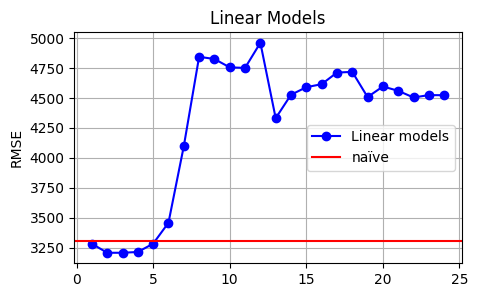
\includegraphics[width=0.95\columnwidth]{C1_LinearModels.png}
            \caption{RMSE de validação dos diferentes modelos testados com o novo conjunto de dados.}
            \label{fig:modelos_lineares_novo}
        \end{figure}

        Foi aplicado o mesmo processo de reconstruir o modelo \emph{ótimo} (com $\textbf{K} = 2$) em todo o conjunto de treino+validação. Também foi construída uma versão deste modelo sem normalizar as variáveis do problema, de forma a melhor analisar os seus coeficientes (figura \ref{fig:coeficientes_novo}). Fica claro que o modelo é próximo do modelo \emph{naïve}, com um peso grande do valor imediatamente anterior, acrescido de um uma \emph{correção} do valor dois meses atrás. Novamente o modelo pode ser interpretado como um média ponderada. A soma dos coeficientes com o valor relativo da constante é aproximadamente a unidade: $ 0.9211 + 0.0778 = 0.9989$. Como esperado, este novo modelo se ajusta melhor aos dados no período da pandemia (figura \ref{fig:ajuste_novo}).

        \begin{figure}[hbt!]
            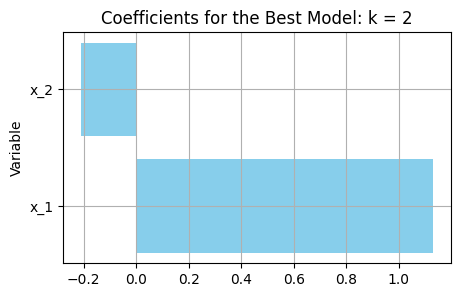
\includegraphics[width=0.95\columnwidth]{C1_CoefficientsNoScaling.png}
            \caption{Coeficientes do novo melhor modelo linear ($\textbf{K} = 2$).}
            \label{fig:coeficientes_novo}
        \end{figure}

        \begin{figure}[hbt!]
            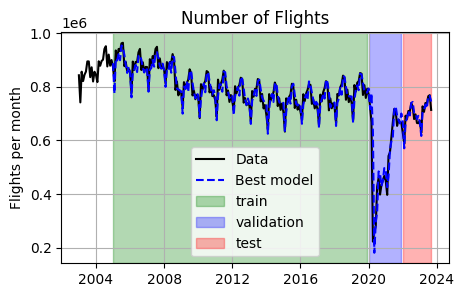
\includegraphics[width=0.95\columnwidth]{C2_BestModelFit.png}
            \caption{Ajuste do novo melhor modelo linear ($\textbf{K} = 2$).}
            \label{fig:ajuste_novo}
        \end{figure}

        Os dados de teste deste novo modelo correspondem aos anos de 2022 e 2023, com valores de erro $\text{RMSE} = 590.57$ e $\text{MAPE} = 0.0208$. Para os anos de 2022 e 2023 os dois modelos construídos mostraram resultados próximos (figuras \ref{fig:erros_modelos} e \ref{fig:ajuste_modelos}), com o primeiro modelo \emph{ligeiramente} melhor..

        \begin{figure}[hbt!]
            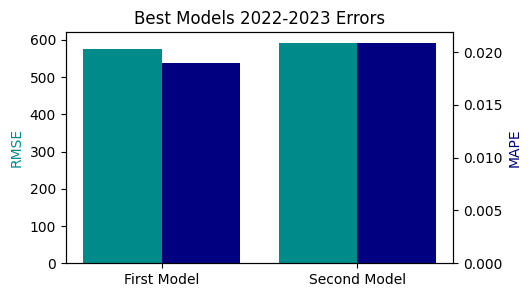
\includegraphics[width=0.95\columnwidth]{C3_RMSE.png}
            \caption{Erros para os dois modelos construídos.}
            \label{fig:erros_modelos}
        \end{figure}

        \begin{figure}[hbt!]
            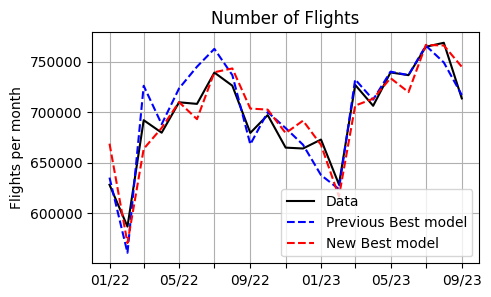
\includegraphics[width=0.95\columnwidth]{C3_BestModel22_23.png}
            \caption{Ajuste em 2022 e 2023 dos dois modelos construídos.}
            \label{fig:ajuste_modelos}
        \end{figure}

        \subsection{Extrapolação Recursiva}

        Para testar a capacidade preditiva destes modelos para um prazo maior, foi feita uma extrapolação recursiva nos períodos de teste, a partir do último valor do período de validação.

        Como esperado, o primeiro modelo não consegue prever o comportamento da série durante a pandemia (figura \ref{fig:extrapolacao_primeiro_modelo}). O modelo apresenta um comportamento \emph{relativamente} estável nesta previsão recursiva. Depois de cerca de um ano o modelo começa a apresentar um comportamento errático, o que coincide com o passo de tempo em que realiza previsões baseadas apena em dados estimados pelo próprio modelo.

        O segundo modelo (figura \ref{fig:extrapolacao_segundo_modelo}), que se baseia unicamente nos dois valores mais recentes, rapidamente perde a capacidade de realizar qualquer previsão confiável.

        Nenhum dos modelos pode ser utilizado para realizar previsões além do mês seguinte. É necessário realizar uma ajuste específico para valores de L maiores que um.

        \begin{figure}[hbt!]
            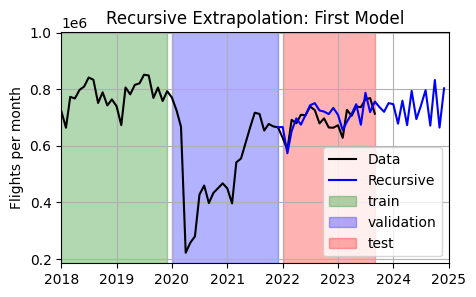
\includegraphics[width=0.95\columnwidth]{C3_RecursiveExtrapolation.png}
            \caption{Extrapolação recursiva com o primeiro modelo.}
            \label{fig:extrapolacao_primeiro_modelo}
        \end{figure}

        \begin{figure}[hbt!]
            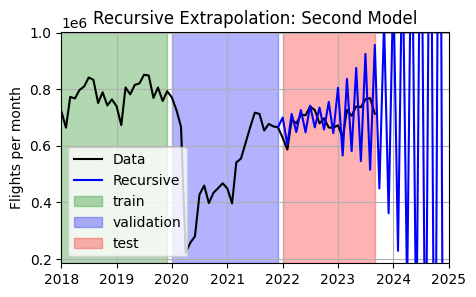
\includegraphics[width=0.95\columnwidth]{C3_RecursiveExtrapolation_new.png}
            \caption{Extrapolação recursiva com o segundo modelo.}
            \label{fig:extrapolacao_segundo_modelo}
        \end{figure}

\section{Conclusão}

    As características dos períodos de treino e validação tiveram impacto no número de parâmetros de cada modelo. A definição dos períodos de teste e validação deve estar alinhada com o que se espera do modelo a ser construído.

    Ambos modelos dependem muito do valor do mês anterior para estimar o próximo, e são incapazes de responder adequadamente a eventos com variações abruptas. Variáveis adicionais são necessárias para permitir que os modelos lineares conseguam aproximar melhor eventos como as restrições impostas pela Pandemia de Covid-19.


\appendix

% \section{Lista de Variáveis}

    % \begin{description}
    %     \item[$X$:] xxxxxxxxxxx.
    % \end{description}


%% \section{}
%% \label{}

%% If you have bibdatabase file and want bibtex to generate the
%% bibitems, please use
%%

\bibliographystyle{elsarticle-num}
\bibliography{refs}

%% else use the following coding to input the bibitems directly in the
%% TeX file.

% \begin{thebibliography}{00}

%% \bibitem{label}
%% Text of bibliographic item

% \bibitem{}

% \end{thebibliography}

% \newpage
% \FloatBarrier
% \section{Código em C}

% O código de ambos métodos foi implementado em um único arquivo. O código é apresentado em duas partes neste documento para facilitar a leitura. O código pode ser encontrado em \href{https://github.com/TiagoCAAmorim/numerical-methods}{https://github.com/TiagoCAAmorim/numerical-methods}.

% \subsection{Método da Bissecção}
% \lstinputlisting[language=C, linerange={1-229}]{./02_newton_raphson.c}

% \subsection{Método de Newton-Raphson}
% \lstinputlisting[language=C, linerange={231-445}]{./02_newton_raphson.c}

% \subsection{Método da Mínima Curvatura}
% \lstinputlisting[language=C, linerange={448-958}]{./02_newton_raphson.c}

\end{document}
\endinput